\section{Eksperimentel opsætning}

\begin{frame}{Eksperimentel opsætning}
	\begin{columns}
		\column{0.4\textwidth}
		\begin{figure}
			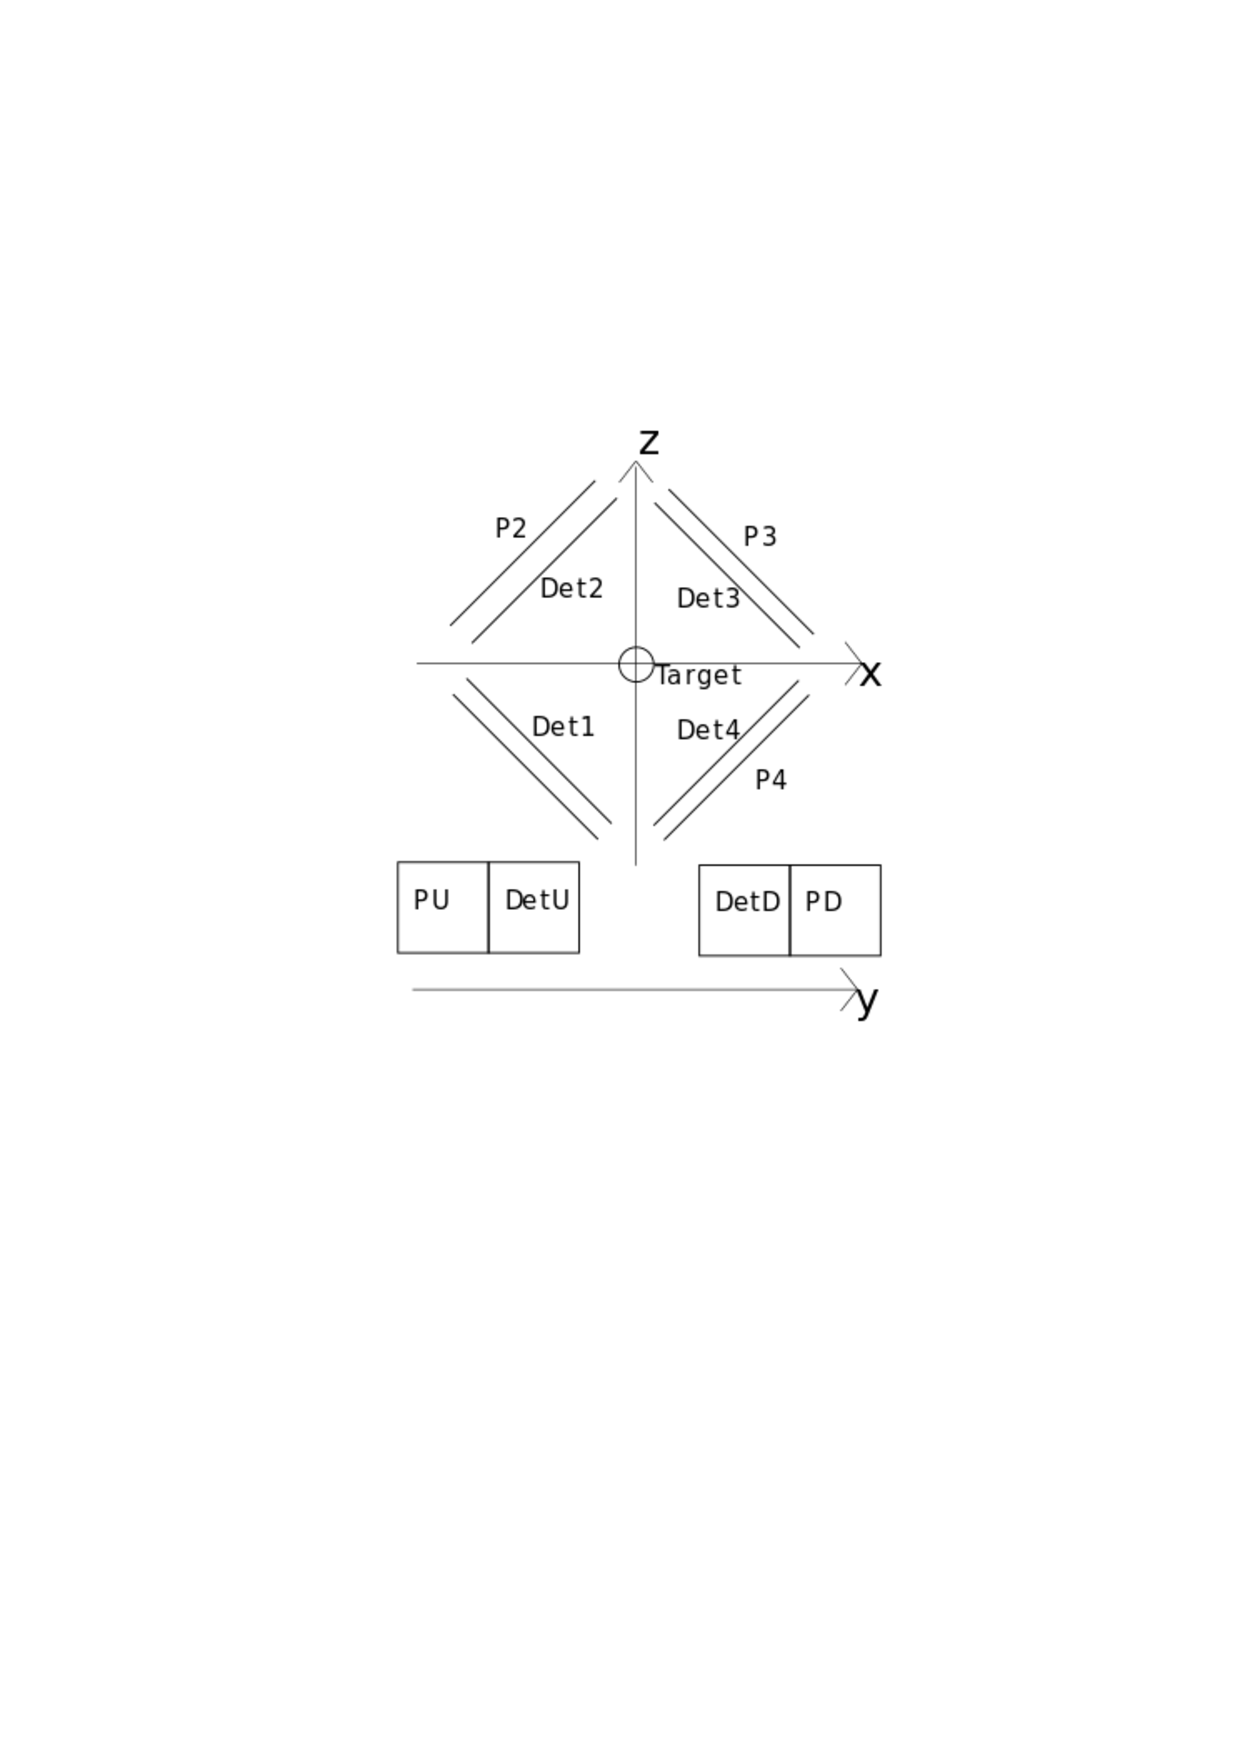
\includegraphics[width=\columnwidth]{../figures/opstilling_better.pdf}
		\end{figure}
		
		\column{0.6\textwidth}
		\small
		\begin{table}
			\begin{tabular}{ll|ll}
				Detektor & Tykkelse {[}$\mu$m{]}  & PAD & Tykkelse{[}$\mu$m{]} 	\\ \hline
				Det1     & 67                     & n/a & n/a                   \\
				Det2     & 1002                   & P2  & 1036                  \\
				Det3     & 65                     & P3  & 1497                  \\
				Det4     & 60                     & P4  & 1490                  \\
				DetU     & 60                     & PU  & 1498                  \\
				DetD     & 1043                   & PD  & 1038                 
			\end{tabular}
		\end{table}		
	\end{columns}


\end{frame}

\begin{frame}{Eksperimentel opsætning}
	\begin{columns}
		\column{0.49\textwidth}
		\begin{figure}
			\centering
			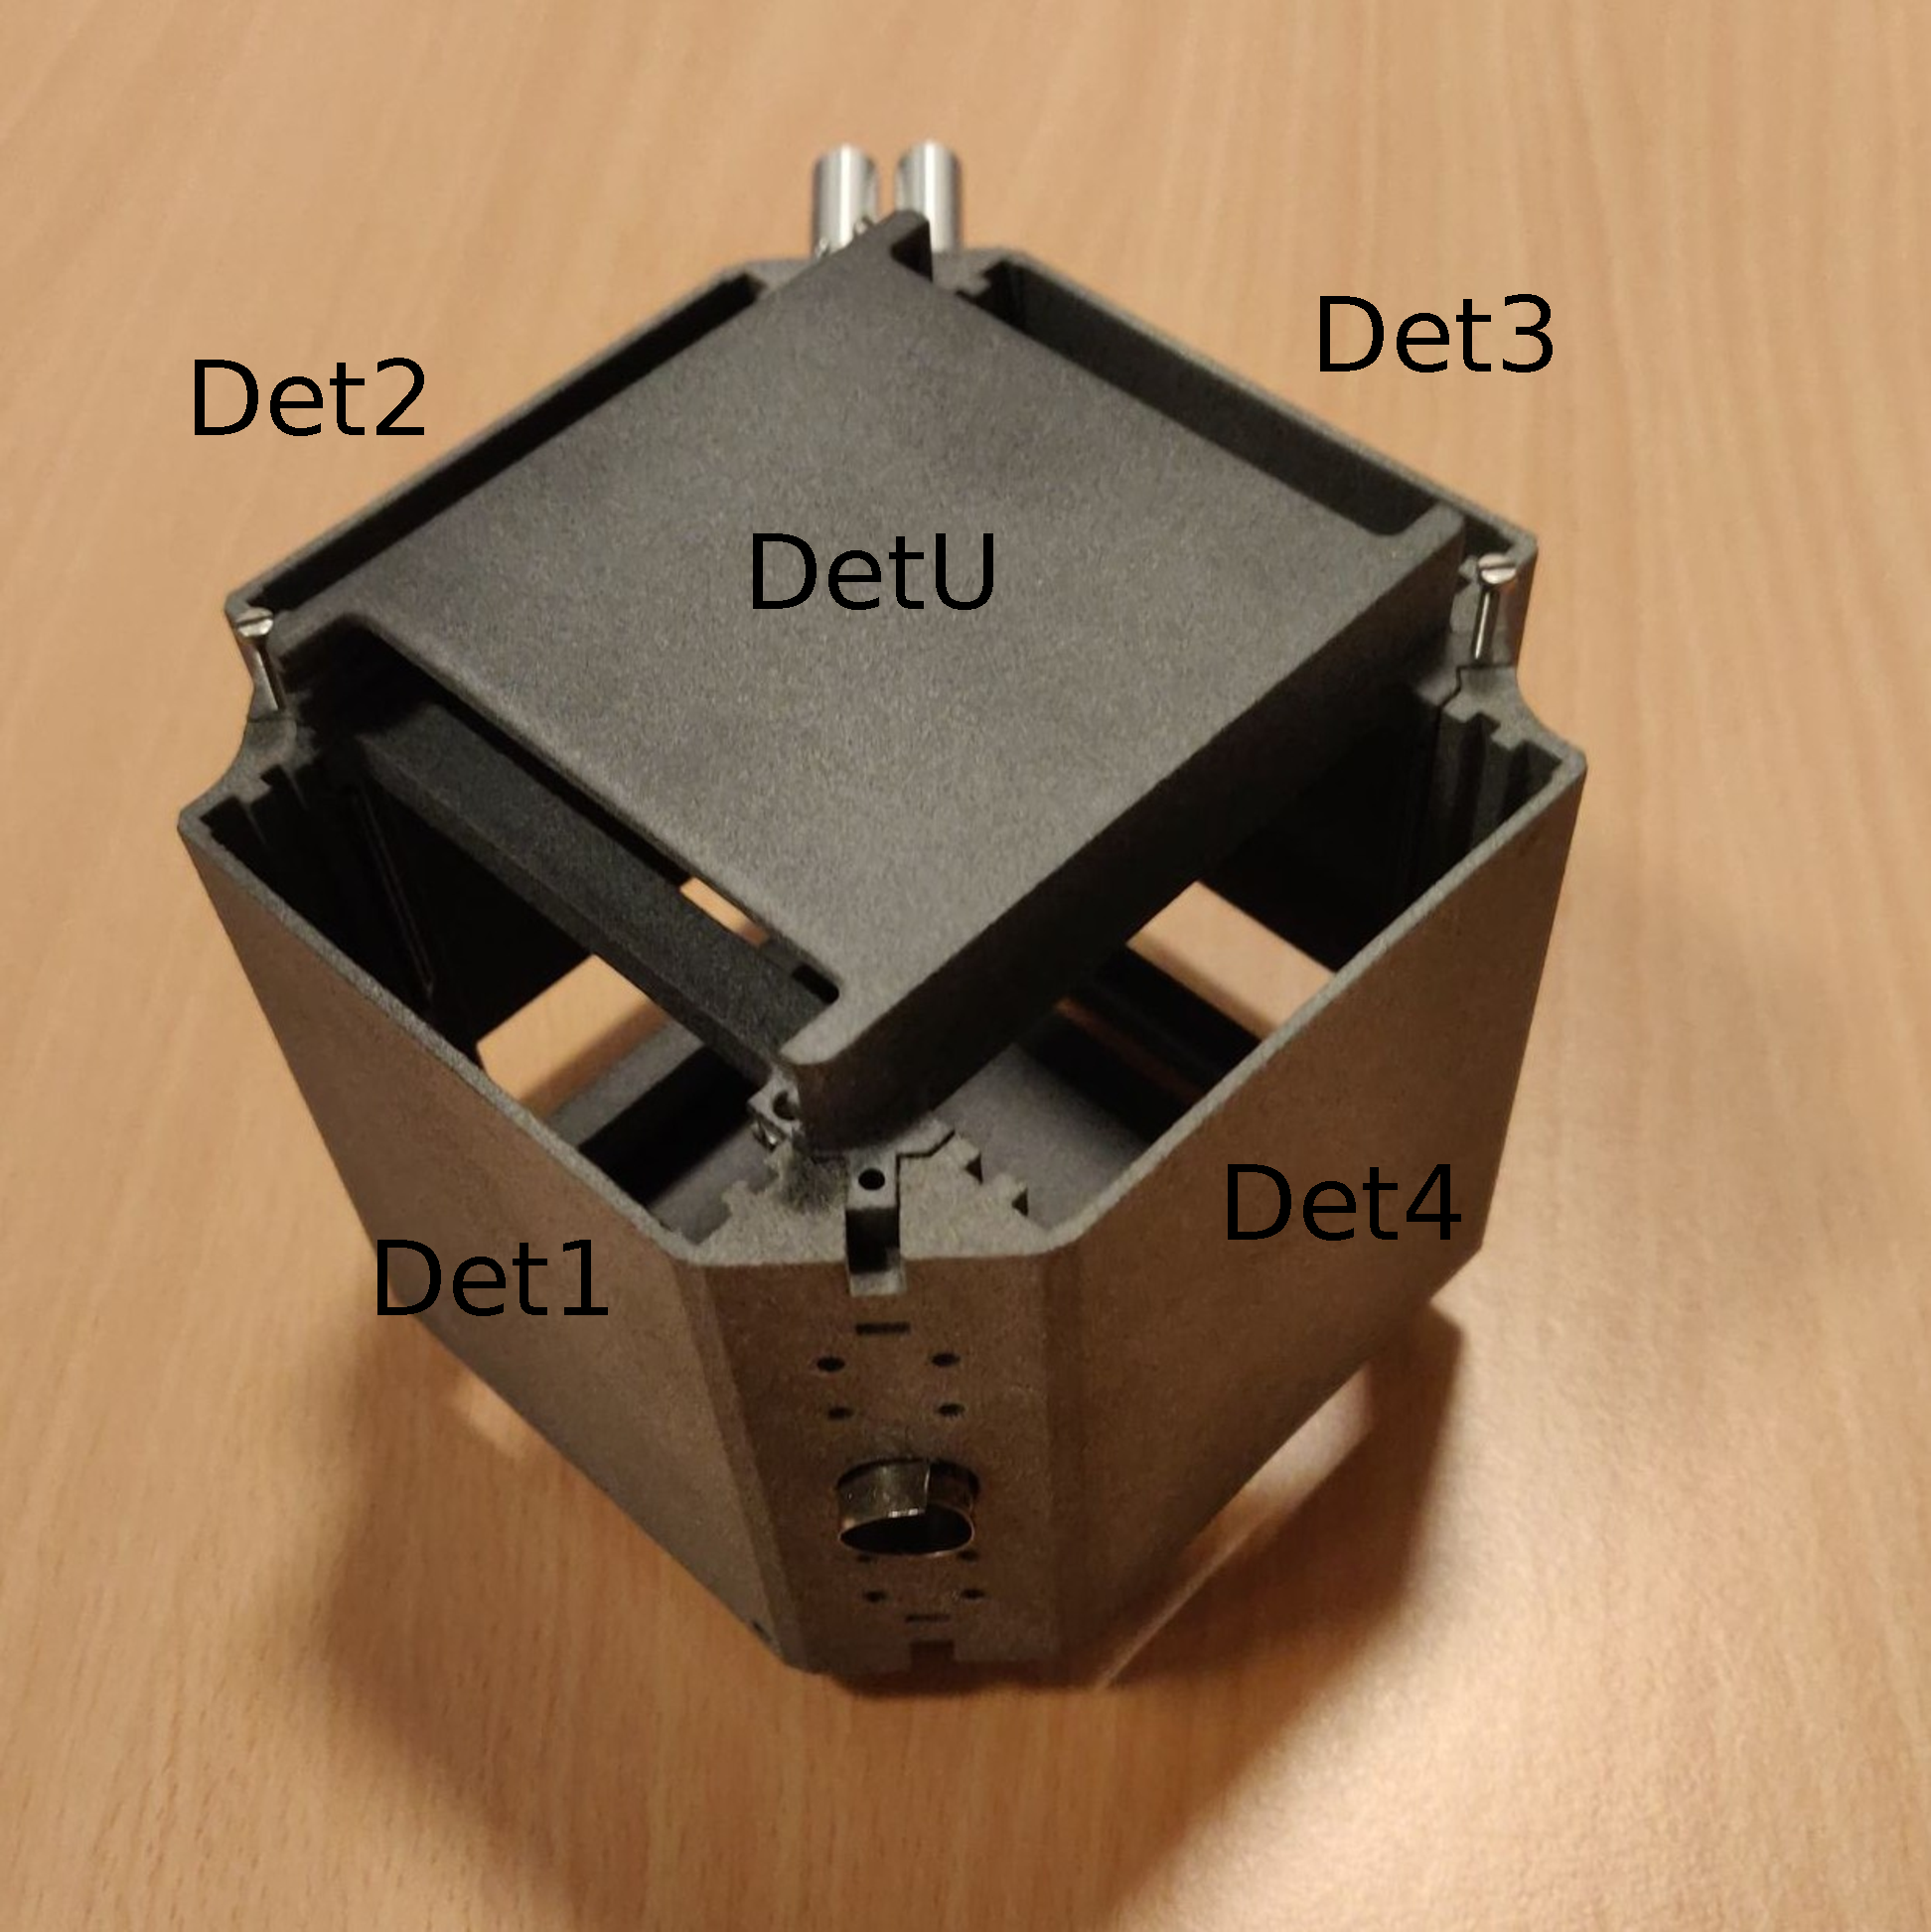
\includegraphics[width=\columnwidth]{../figures/cubepic.pdf}
		\end{figure}
		\column{0.49\textwidth}
		\begin{figure}
			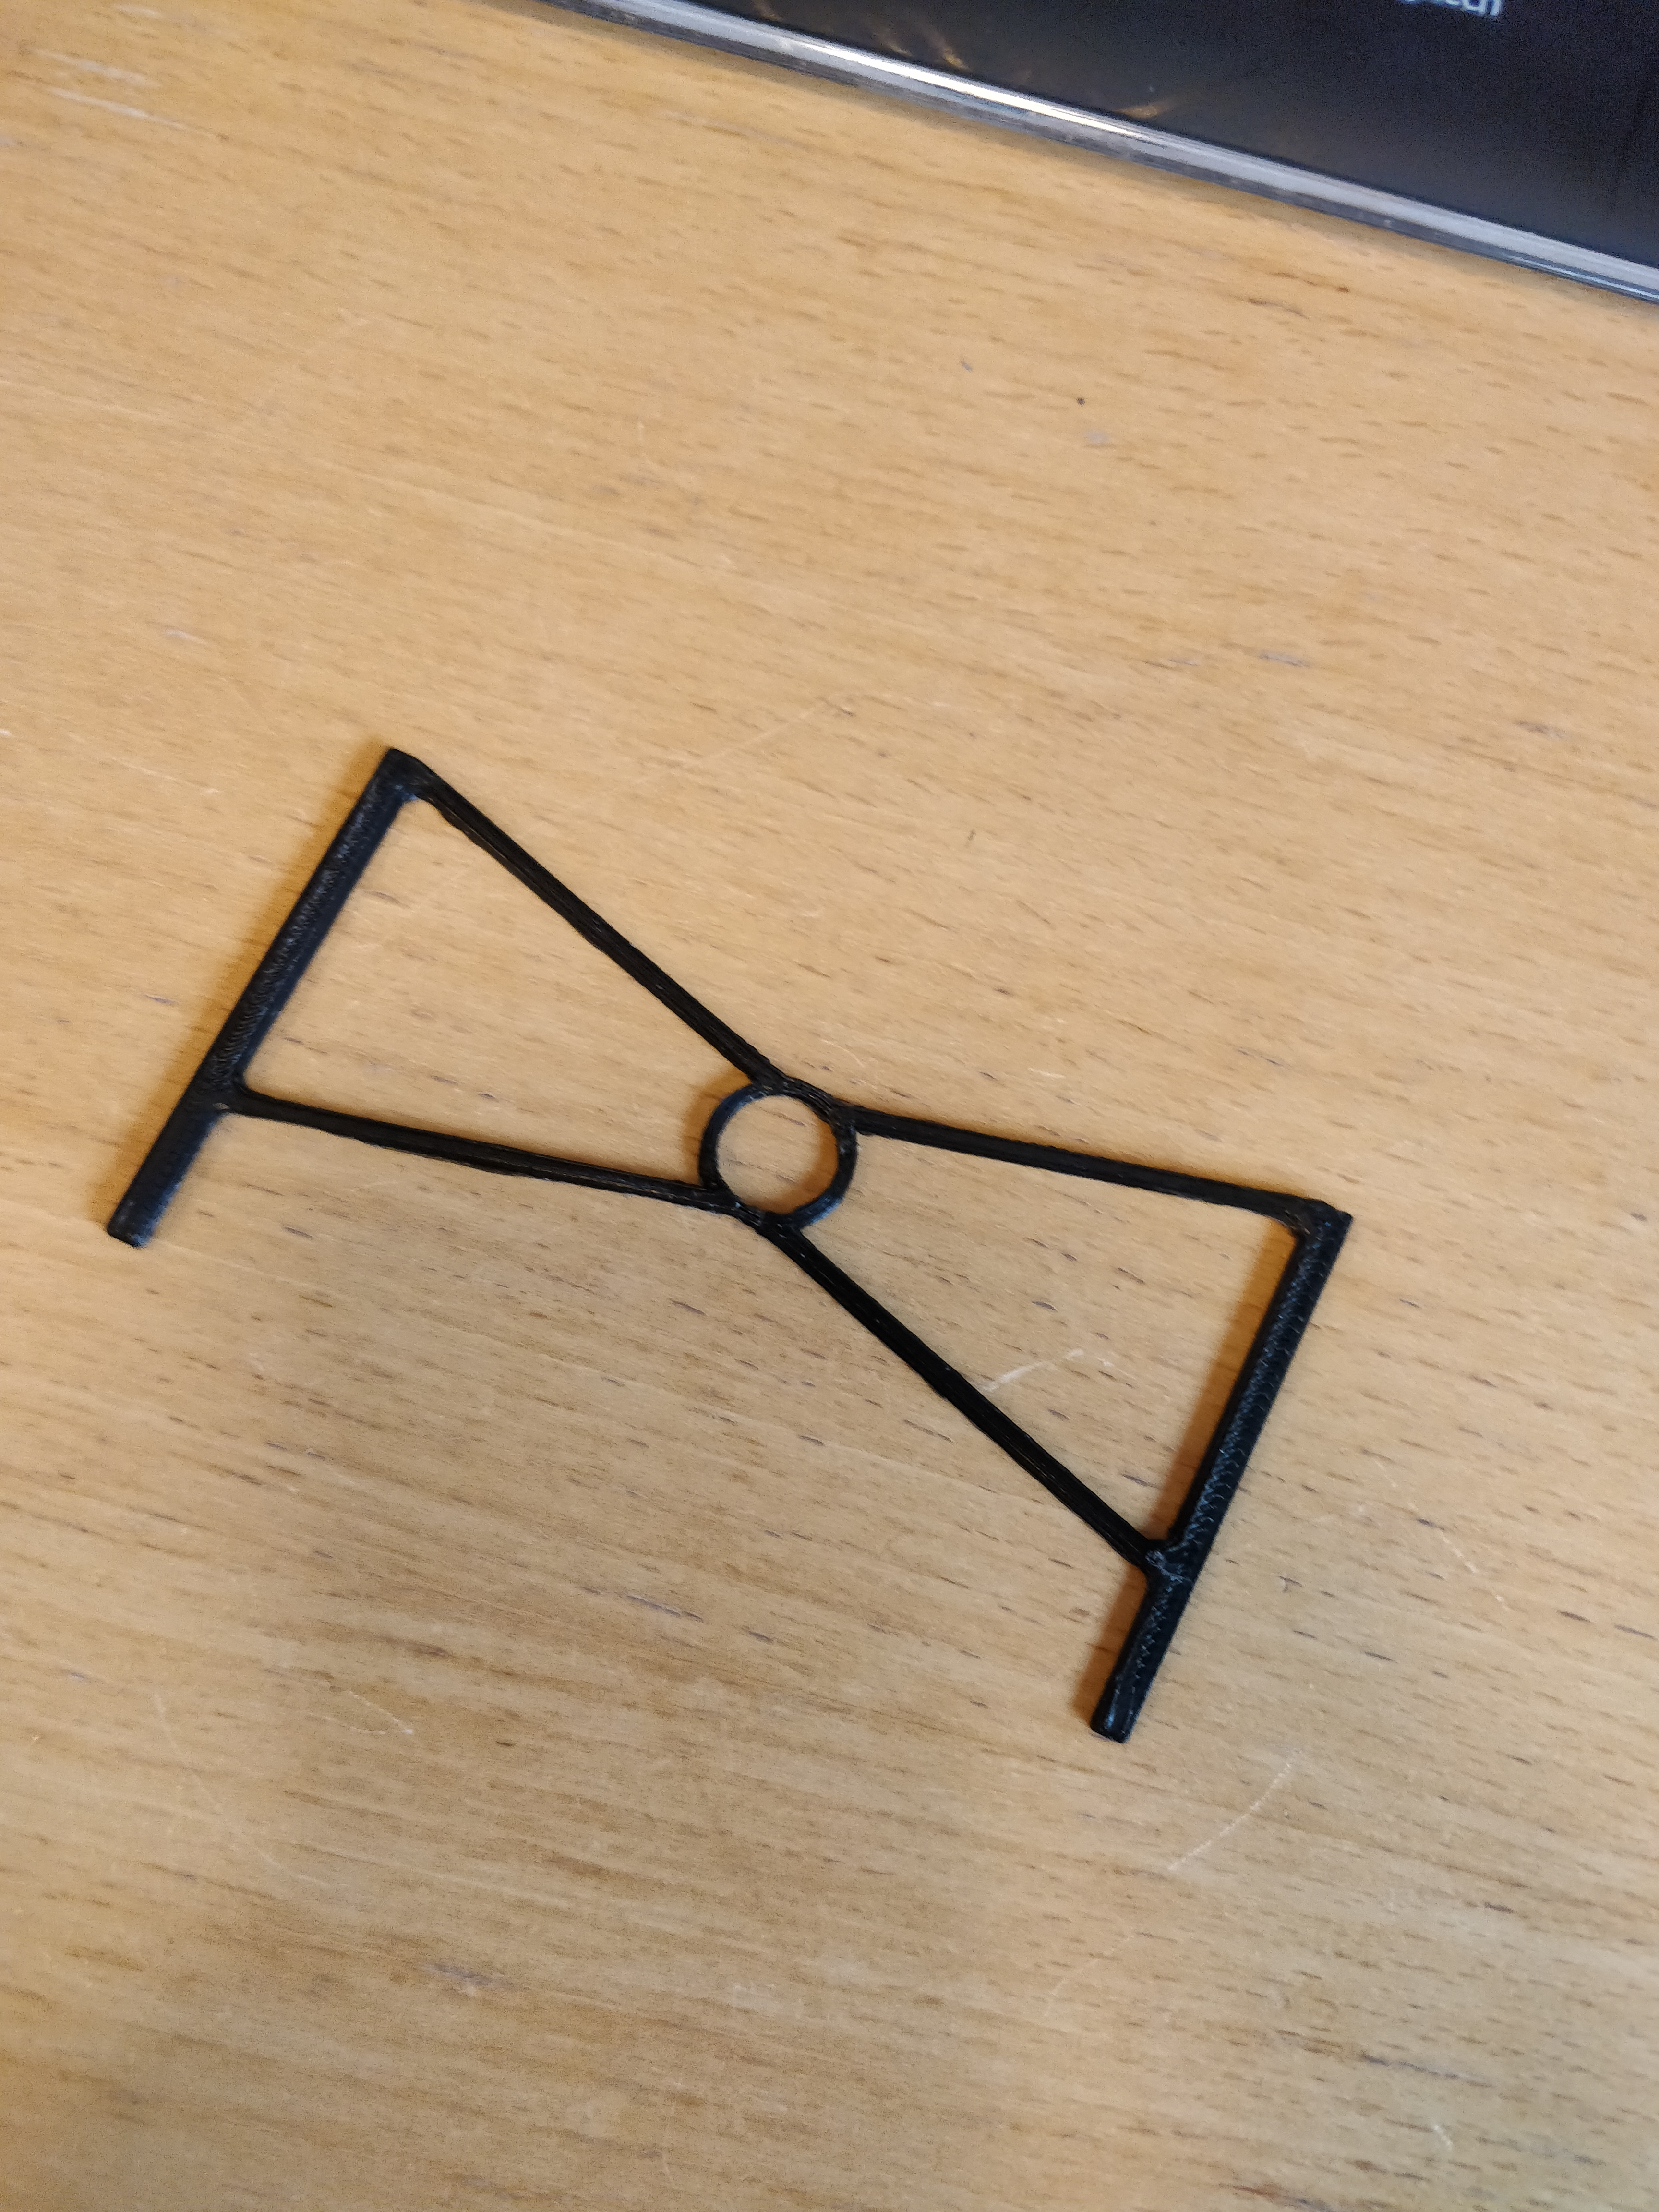
\includegraphics[width=.9\columnwidth]{../figures/targetHolder.jpg}
		\end{figure}
	\end{columns}
\end{frame}

\begin{frame}{Detektorerne}
	\begin{columns}
		\column{0.4\textwidth}
		\begin{figure}
			\centering
			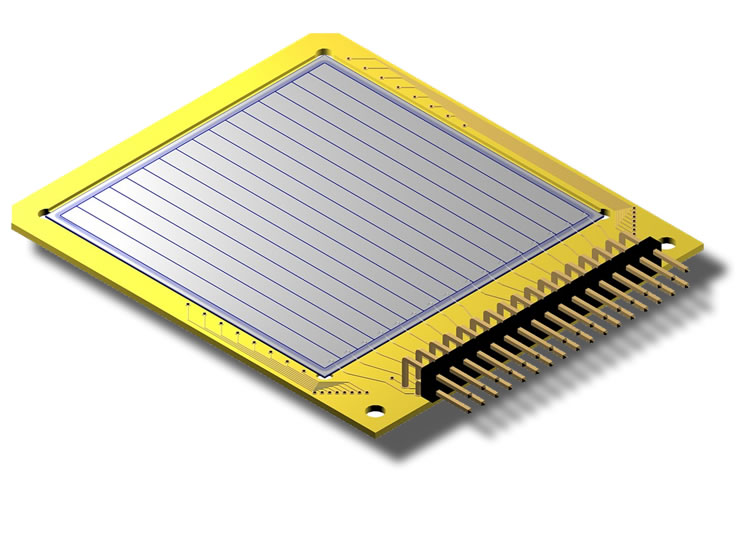
\includegraphics[width=\columnwidth]{../figures/W1.jpg}
		\end{figure}
		$16\times16$ strips\\
		256 pixels 
		\column{0.6\textwidth}
		\begin{figure}
			\centering
			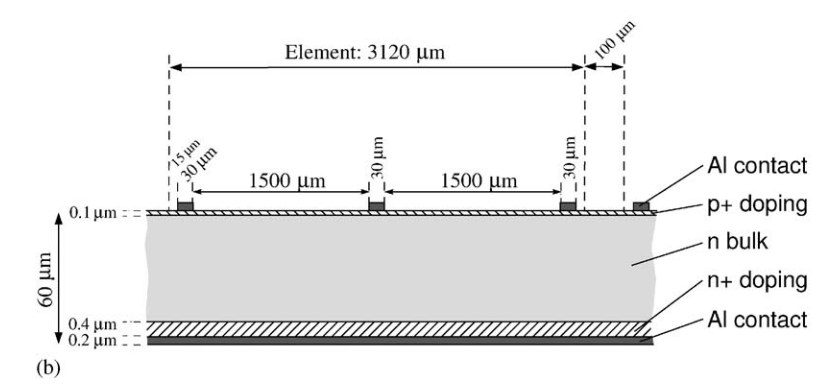
\includegraphics[width=\columnwidth]{../figures/dope.png}
		\end{figure}
	\end{columns}
\end{frame}

\begin{frame}{Software}
	\begin{columns}
		\column[]{0.6\textwidth}
	\begin{itemize}
		\onslide<2->{\item ROOT}
		\begin{itemize}
			\onslide<3->{\item C++ framework}
		\end{itemize}
		\onslide<4->{\item AUSA}
		\begin{itemize}
			\onslide<5->{\item Unpacker: Rå data til ROOT \texttt{Tree}}
			\onslide<6->{\item Calibrator: Detektor kalibrering}
			\onslide<7->{\item Sorter: Konvertere strip signaler til pixel hit}
		\end{itemize}
	\end{itemize}
	\column[]{0.4\textwidth}
	\onslide<7->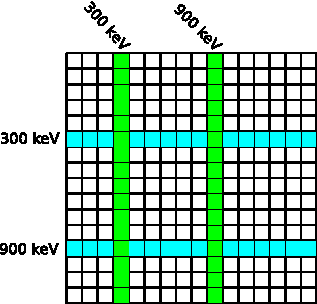
\includegraphics[width=\columnwidth]{../figures/sorter.pdf}
\end{columns}
\end{frame}

\begin{frame}{Kalibrering}
	\begin{columns}
		\column{0.5\textwidth}
		Konverter kanal nummer til en energi
		Kendte kilder:\\
		\begin{table}[H]
			\centering
			\begin{tabular}{ll}
				Isotope & $E_\alpha \ [keV]$  \\ \hline
				\isotope[148][]{Gd}		& 3182.690         \\
				\isotope[239][]{Pu}		& 5105.5           \\
				& 5144.3           \\
				& 5156.59          \\
				\isotope[244][]{Cm}		& 5762.64          \\
				& 5804.96          \\ 
			\end{tabular}
		\end{table}
	
		\column{0.5\textwidth}
		\begin{figure}
			\centering
			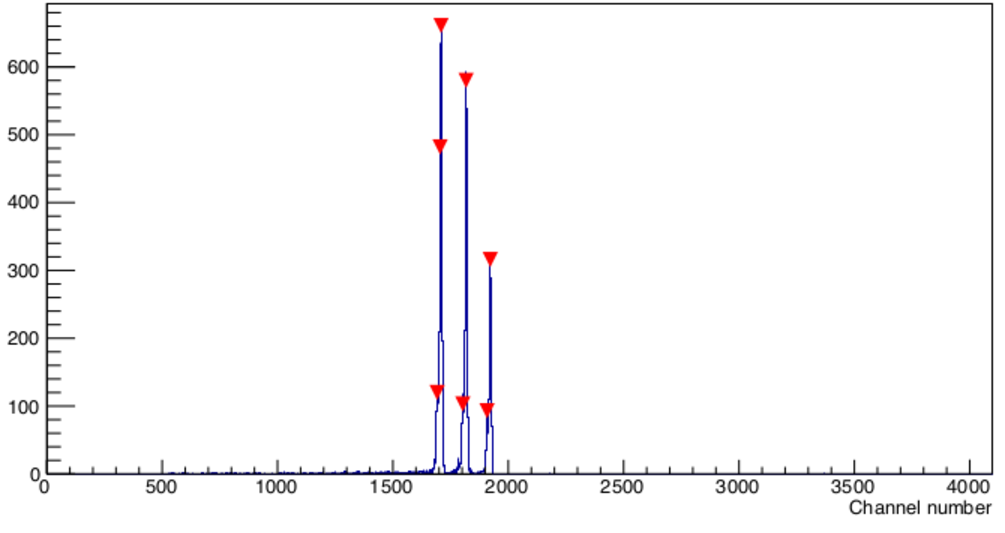
\includegraphics[width=\columnwidth]{../figures/cali/det1f1-cropped-Mia.pdf}
		\end{figure}
		\begin{figure}
			\centering
			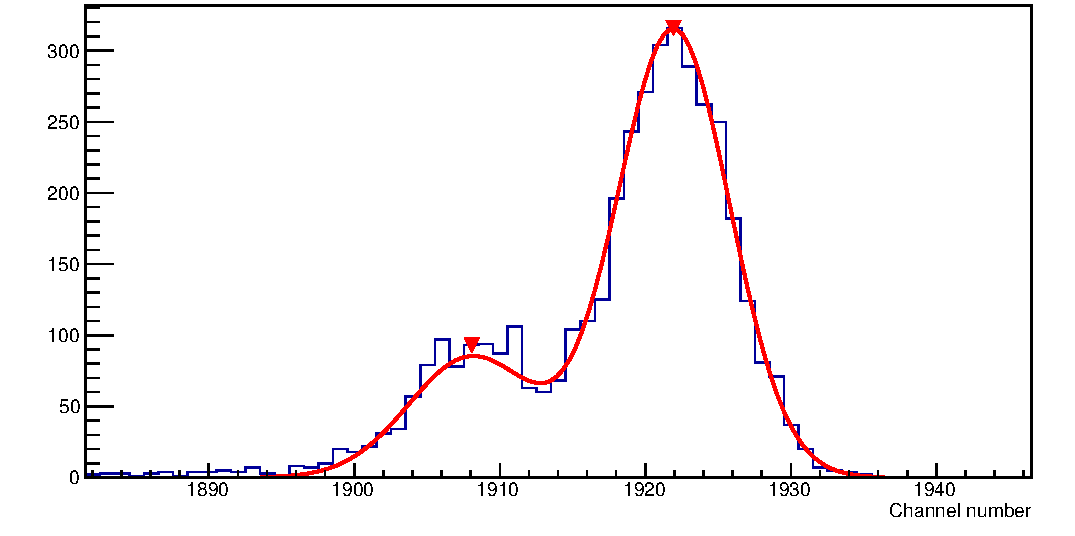
\includegraphics[width=\columnwidth]{../figures/cali/det1f1PeakMostLeft-cropped.pdf}
		\end{figure}
	\end{columns}
\end{frame}

